% !TEX root = BA-Bauer.tex

\subsection{Aufnahmefunktionen}
\label{sec:recfunctions}
Für die Aufnahme von DMX-Daten stehen insgesamt vier verschiedene Aufnahmemodi zur Verfügung, welche jeweils eine Aufnahmefunktion bilden. Der erste Aufnahmemodus ist der Standard-Modus, bei dem vorab die Dauer der Aufnahme festgelegt wird. Nach Ablauf der Aufnahmedauer stoppt die Aufnahme und kehrt zum Menü zurück. Der zweite Modus ist der sogenannte $Trigger$-Modus, bei dem zuvor in den Einstellungen ein $Trigger$-Kanal und $Trigger$-Wert festgelegt wird. Ist die Aufnahme gestartet und in den eingehenden DMX-Datenpaketen wird der $Trigger$-Wert des ausgewhählten $Trigger$-Kanals überschritten, so startet ab diesem Zeitpunkt die Speicherung der DMX-Daten. Die Aufnahme wird gestoppt, wenn der $Trigger$-Wert wieder unterschritten wird. Dieser Modus ermöglich das Starten und Stoppen der Aufnahme zu sehr präzisen Zeitpunkten. Vor allem für sich wiederholende Bewegungsabläufe von Lichttechnischen Geräten ist diese Funktion äüßerst sinnvoll. Ist die Position eines Lichtkegels beispielsweise am Anfang und Ende der Aufnahme identisch, so kann die Aufnahme endlos nacheinander wiedergegeben werden, ohne dass ein Anfang oder Ende der aufgenommenen Sequenz sichtbar ist. Der letzte kontinuierliche Aufnahme-Typ ist die endlose Aufnahme, bei der die Aufnahme ohne die Wahl einer Aufnahmedauer gestartet wird und durch betätigen des Zurück-Tasters gestoppt wird. Dieser Modus richtet sich an Situationen, in denen die Endzeit der Aufnahme beim Aufnahmebeginn nicht festgelegt werden kann. Ein Beispiel für einen Anwendungsfall ist ein Konzert. Zu beginn des Konzerts kann die Aufnahme gestartet werden und nachdem die letzte Zugabe gespielt ist, wieder gestoppt werden. Bei dem letzten Aufnahme-Typ handelt es sich um eine nicht-kontinuierliche Aufnahme der DMX-Daten, die sogenannte $Step$-Aufnahme. Bei diesem Aufnahme-Typ können einzelne Datenpakete des eingehenden DMX-Datenstroms aufgenommen werden. Jedes Datenpaket entspricht einem $Step$ und enthält, im Gegensatz zu den drei anderen Aufnahmemodi, keine Zeitinformationen. Die einzelnen Steps werden bei der Wiedergabe in einem regelmäßigen Zeitabstand, der erst bei der Wiedergabe vom Benutzer festgelegt wird, wiedergegeben. Dieser Modus gibt dem Benutzer die Möglichkeit die DMX-Datenpakete in einer bestimmten Taktung auszugeben und diese beispielweise an den Takt eines Liedes anzupassen. Zudem wird durch die Speicherung einzelner Datenpakete, im Vergleich zu den anderen Aufnahmemodi, deutlich weniger Speicherplatz auf der SD-Karte benötigt. 
Im Folgenden wird auf das Grundprinzip der Aufnahmefunktionen eingegangen. Ein Flussdiagramm des Standard-Aufnahmemodus befindet sich im Anhang \ref{fluss:recf}.\newline
Die drei Aufnahmemodi der kontinuierlichen Aufnahme, also Standard-, Endlose- und $Trigger$-Aufnahme unterscheiden sich im wesentlichen nur in den Start- bzw. Stoppbedingungen, welche in Tabelle \ref{tab:recstartstop} zusammengefasst sind. Im Standardmodus muss zusätzlich eine Aufnahmezeit festgelegt werden. 
\begin{table}[h]
	\begin{center}
		\caption{Start und Stoppbedingungen der Aufnahmemodi}
		\label{tab:recstartstop}
		\begin{tabular}{l | p{6cm} | p{6cm}}
			Modus & Startbedingung & Stoppbedingung\\
			\hline
			Standard & Bestätigungstaster & Ablauf der Aufnahmezeit\\
			Endlos & Bestätigungstaster & Zurück-Taster\\
			$Trigger$ & $Trigger$-Wert auf $Trigger$-Kanal überschreiten & $Trigger$-Wert auf $Trigger$-Kanal unterschreiten
		\end{tabular}
	\end{center}
\end{table}\newline
\subsubsection{Festlegen der Aufnahmezeit}
Abbildung \ref{lcd:rectime} zeigt die Ausgabe auf dem LCD-Display für die Festlegung der Aufnahmezeit. Die Auswahl der Zeit ist in vier Blöcke für das Einstellen der Stunden, Minuten, Sekunden und Millisekunden aufgeteilt. Mit den Links- und Rechts-Tastern kann der ausgewählte Block, markiert mit dem Zeichen in der untersten Zeile des Displays, verändert werden. 
\begin{figure}[h]
	\begin{center}
		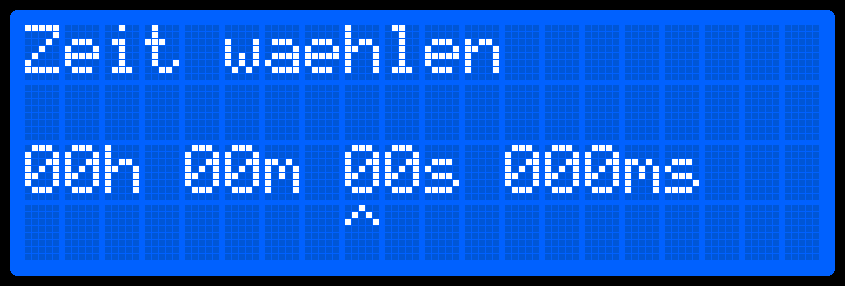
\includegraphics[width=.25\linewidth]{LCD-Screenshots/Zeitauswahl}
		\caption{LCD-Ausgabe Aufnahmezeit}
		\label{lcd:rectime}
	\end{center}
\end{figure}
Der Wert des Blocks wird mit einer Drehung des Encoders im Uhrzeigersinn erhöht und gegen den Uhrzeigersinn verringert. Der Millisekunden-Block erhöht, bzw. verringert sich immer um 10 Millisekunden. Eine feinere Auflösung im Millisekundenbereich ist nicht sinnvoll, da die DMX-Datenpakete eine Zeitdauer von 22\,ms zur vollständigen Übertragung benötigen. Wird eine Drehbewegung des Encoders registriert, so wird zunächst überprüft ob der vorherige Wert weiter erhöht oder verringert werden kann. Damit wird ausgeschlossen, dass eine Zeit kleiner null gewählt werden kann oder beispielsweise die Anzahl der Minuten größer 59 ist. Ist die Auswahl der Zeit beendet so muss sie mit dem Bestätigung-Taster bestätigt werden. Die eingegebene Zeit wird dann in Millisekunden umgerechnet und in die entsprechende Variable der Aufnahmezeit geschrieben.\\
\newline
\textbf{Optimierungsmöglichkeiten}\\
Um die Festlegung der Aufnahmezeit noch Benutzerfreundlicher zu gestalten, ist es sinnvoll die Begrenzungen der einstellbaren Zeit aufzuheben. Sind zum Beispiel 59\,Sekunden eingestellt und der Wert wird mit einer Drehung des Encoder weiter erhöht, so wäre es sinnvoll die Anzahl der Minuten zu inkrementieren und die Anzahl der Sekunden auf null zurückzusetzten. Das gleich Prinzip könnte auch in die andere Richtung funktionieren. Außerdem ist bei der Festlegung der Zeit die maximal mögliche Aufnahmedauer nicht berücksichtigt. Der Benutzer hätte also die Möglichkeit eine Aufnahmezeit festzulegen, die technisch aufgrund der maximalen Dateigröße auf der SD-Karte nicht erreicht werden kann. Dieser Fall sollte durch eine entsprechende Abfrage abgefangen werden.
\subsubsection{Festlegen des Dateinamens}
Jede Aufnahme erfordert die Festlegung eines Dateinamens um eine Auswahl bei der Wiedergabe zu ermöglichen. Der vor der Aufnahme festgelegte Name entspricht dem Dateinamen der Datei auf der SD-Karte und ermöglicht dem Benutzer ausgewählte Aufnahmen auf andere SD-Karten zu übertragen oder Sicherheitskopien anzulegen. Dem Benutzer stehen bei der Festlegung des Namens insgesamt acht Zeichen zur Verfügung. Abbildung \ref{lcd:filename} zeigt die Ausgabe auf dem LCD-Display. Wie bereits im vorherigen Kapitel, wird mithilfe der Links- und Rechts-Taster eine Auswahl getroffen, in diesem Fall ein Zeichen des Dateinamens. Durch drehen des Encoders können die Zeichen geändert werden. Verfügbare Zeichen sind alle Buchstaben von A-Z in kleiner und großer Schreibweise, Zahlen von 0-9, sowie ein Leerzeichen und ein Unterstrich.
\begin{figure}[h]
	\begin{center}
		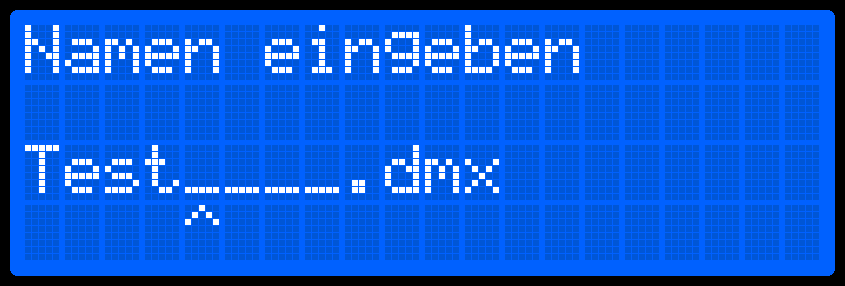
\includegraphics[width=.25\linewidth]{LCD-Screenshots/Namenauswahl}
		\caption{LCD-Ausgabe Dateinamen einstellen}
		\label{lcd:filename}
	\end{center}
\end{figure}
Umgesetzt wird dieser Programmteil mithilfe eines Zeichen-Arrays, dessen Anzahl an Zellen der Länge des Dateinamens entspricht. Die letzten vier Zellen des Arrays werden mit der Dateiendung ($.dmx$) beschrieben. Die Endung ist bei der Auswahl des Namens nicht veränderbar. Die restlichen Zellen des Arrays werden inital mit einem Unterstricht beschrieben und sollen damit dem Benutzer ein veränderbares Zeichen signalisieren. Ein Zeichen besteht aus einem Byte und kann somit 256 Werte annehmen, wobei jeder Wert einem Zeichen entspricht. Wird zum Beispiel der Wert der einem $a$ entspricht um 1 inkrementiert, so wird ein $b$ dargestellt. Aufgrund dieses Systems kann der Wert der Position des Encoder unmittelbar als Zeichen dargestellt werden und in die entsprechende Zelle des Arrays geschrieben werden. Eine Veränderung der Encoderposition bewirkt eine Änderung des gerade ausgewählten Zeichens.
% !TEX root = BA-Bauer.tex

\subsubsection{Aufnahme eines DMX-Datenpaketes}
Die Aufnahme eines DMX-Datenpaketes zählt zu den kritischsten Zeilen Programmcode dieser Arbeit. Wird das erste Datenbyte nicht registriert, hat das bei der Wiedergabe, aufgrund der seriellen Übertragung des DMX-Protokolls, Auswirkungen auf alle angeschlossenen Geräte. Das Prinzip der Aufnahme von DMX-Datenpaketen ist bereits in der Praxisprojektarbeit aufgezeigt und wird in dieser Arbeit optimiert.
Die Aufnahme eines Datenpaketes basiert auf den Interrupt-Events der UART-Schnittstelle. Bei jedem empfangenen oder gesendetem Datenbyte, erkannten Fehler der Übertragung oder der Schnittstelle wird ein globaler Interrupt ausgelöst. In der aufgerufenen Funktion wird identifiziert was den Interrupt ausgelöst hat und es wird ein entsprechender Code ausgeführt. Für die Aufnahme sind die Events des $Framing\ Errors$ und des erfolgreichen Empfangs eines Datenbytes von Bedeutung. Wie in der Praxisprojektarbeit wird mithilfe des $Framing\ Errors$ das Ende eines DMX-Datenpaketes erkannt. Codeausschnitt \ref{code:itSaveByte}, \ref{code:dmx.c-rxIT}, \ref{code:itFE}, \ref{code:itErrorclear} und \ref{code:itResetRx} zeigen Ausschnitte aus der globalen UART-Interruptfunktion, die wesentlich für den Empfang von DMX-Datenpaketen sind. Die folgende Funktion wird aufgerufen wenn ein Datenbyte ohne einen Fehler vollständig empfangen und bereit zum Lesen ist. 
\begin{lstlisting}[caption = stm32f4xx\_it.c: UART Save\_Byte\_Rx(),
label = code:itSaveByte, 
language = C, 
firstnumber = 442]
static void Save_Byte_Rx()
{
	*huart4.pRxBuffPtr++ = huart4.Instance->DR; //DR in Buffer speichern
	if(--huart4.RxXferCount == 0U)
	{
		//save to SD
		HAL_UART_RxCpltCallback(&huart4);
		Reset_Rx();
	}
}
\end{lstlisting}
Zunächst wird in Zeile 444 das eingegangene Datenbyte aus dem $DR$-Register der UART-Schnittstelle dem Zeiger auf das Puffer-Array (\textit{huart4.pRxBuffPtr}) zugewiesen und dieser anschließend um einer Stelle inkrementiert.
Darauf folgt eine $if$-Abfrage, die Identifiziert, ob alle erwarteten Datenbytes empfangen sind. Bei einem Aufruf der Empfangsfunktion $HAL\_UART\_Receive\_IT(...)$ zum Starten des Empfangsvorgangs der UART-Schnittstelle wird die Anzhal der zu empfangenen Datenbytes der Vaiable $RxXferCount$ zugewiesen und wird bei jedem empfangenen Datenbyte um eine Stelle dekrementiert. Enthält die Variable nach der Dekrementierung den Wert 0, so sind alle Datenbytes empfangen und ein entsprechender $Callback$ wird aufgerufen. Dieser befindet sich in der Datei $DMX.c$ und ist in Codeausschnitt \ref{code:rxIT} zu sehen. 
\lstinputlisting[
caption = DMX.c: Callback-Funktion eingehender UART-Daten,
label = code:dmx.c-rxIT, 
language = C, 
firstnumber = 103, 
firstline = 103, 
lastline = 113]
{/Users/Felix/Documents/CubeMX/BPA-Code/Core/Src/DMX.c}
Wenn die Callback Funktion aufgerufen wird, ist ein DMX-Datenpaket vollständig empfangen. Dem Hauptprogramm wird das mithilfe der Zuweisung der Variable $RxComplete$ mit dem Wert 1 signalisiert. Die Variable der Anzahl der empfangenen Datenpakete $received\_packets$ wird außerdem inkrementiert. Das Ein- bzw. Ausschalten der Empfangs-LED ($LED\_RX$) gibt dem Benutzer eine Rückmeldung über den erfolgreichen Empfang eines DMX-Datenpaketes. Ist durch das Hauptprogramm die Variable $recording$ nicht mit dem  Wert 1 beschrieben, also findet keine aktive Speicherung der Daten statt, wird die Status-LED ein- bzw. ausgeschaltet. Der Benutzer bekommt somit eine Rückmeldung über den Datenfluss bevor eine Aufnahme aktiv gestartet wird. Somit kann sichergagengen werden, dass DMX-Daten fehlerfrei eingehen und bei einem Start der Aufnahme keine unerwarteten Fehler im Bezug auf den Datenfluss auftreten.
\newline
Nach der Bearbeitung des Callbacks wird als letzter Schritt die Funktion $Reset\_Rx()$ (Codeausschnitt \,\ref{code:itResetRx})aufgerufen. In ihr werden alle Variablen der UART-Schnittstelle auf die für den Empfang eines neuen DMX-Datenpaketes benötigten Initialwerte zurückgesetzt.
\begin{lstlisting}[caption = stm32f4xx\_it.c: UART Reset\_Rx(),
	label = code:itResetRx, 
	language = C, 
	firstnumber = 434]
	static void Reset_Rx()	//Rx complete or Error ->dmx-brake
	{
		huart4.RxXferCount = 513;
		huart4.RxXferSize = 513;
		huart4.pRxBuffPtr = Univers.RxBuffer;
		(void)*huart4.pRxBuffPtr--;
	}
\end{lstlisting}
Das zweite wichtige Event der UART-Schnittstelle ist der $Framing-Error$ ($FE$) der das Ende des DMX-Datenpaketes signalisiert. Codausschnitt \ref{code:itFE} zeigt den Auschnitt der Behandlung eines $FE$ in der globalen Interrupt-Funktion der UART-Schnittstelle. Wird ein $FE$ identifiziert, so muss zunächst das Bit, welches den Error anzeigt zurückgesetzt werden damit die Funktion nicht unmittelbar nach dem Beenden ernuet aufgerufen wird.
\begin{lstlisting}[caption = stm32f4xx\_it.c: UART Framing Error,
	label = code:itFE, 
	language = C, 
	firstnumber = 349]
/* UART frame error interrupt occurred -----------------------------------*/
if (((isrflags & USART_SR_FE) != RESET) && ((cr3its & USART_CR3_EIE) != RESET))
{
	Clear_Rx_Error();
	huart4.ErrorCode |= HAL_UART_ERROR_FE;
}
\end{lstlisting}
Mithilfe der Funktion $Clear\_Rx\_Error()$, dessen Inhalt Codesausschnitt \ref{code:itErrorclear} zeigt, wird druch einen Lesevorgang des entsprechenden Status-Registers $SR$ und des Daten-Registers $DR$ alle gesetzten Bits auf den Initialwert zurückgesetzt. Anschließend wird die Funktion $Reset\_Rx()$ aufgerufen. Zuletzt wird der $ErrorCode$ der UART-Schnittstelle mit dem entsprechenden $FE$ Error-Code beschrieben. 
\begin{lstlisting}[caption = stm32f4xx\_it.c: UART Clear\_Rx\_Error(),
	label = code:itErrorclear, 
	language = C, 
	firstnumber = 426]
static void Clear_Rx_Error()
{
	uint16_t tmp = huart4.Instance->SR;
	tmp = huart4.Instance->DR;
	(void) tmp;
	Reset_Rx();
}
\end{lstlisting}
Dieser Ablauf findet außerdem bei allen anderen auftretenden Fehlern statt um fehlerhafte Datensätze zu verhindern. Nur wenn ein vollständiges Datenpaket empfangen ist oder das Datenpaket durch einen $FE$ als beendet erklärt ist, wird dieses für die Speicherung dem Hauptprogramm \"freigegeben\".\\
\newline
\textbf{Optimierungsmöglichkeiten}\\
Aus progammatischer Sicht ist die Verteilung des Codes über mehrere Dateien nicht besonders elegant und erschwert die Implementierung in zukünftigen Projekten. Besser wäre es den Code vollständig in den Dateien DMX.c und DMX.h unterzubringen. Das erleichtert die Übersichtlichkeit des Programms und beugt damit Fehlern vor. Zudem ist es sinnvoll jeden der bei der Übertragung auftretenden Fehler anders zu behandeln um z.B. eine Fehlerkorrektur durchzuführen und unnötig großen Datenverlust zu verhindern. Anstatt ein komplettes Datenpaket zu ignorieren sobald ein Byte fehlerhaft ist, könnte der Wert des Fehlerhaften Bytes aus dem vorherigen Datenpaket übernommen werden. Damit reduziert sich der Datenverlust von einem Datenpaket auf ein eventuell falsches Daten-Byte. Entsprechende Infomationen über den Anteil von Fehlerhaften Datenpaketen ober -Bytes könnten für den Benutzer ersichtlich dargestellt werden und eine Rückmeldung über die generelle Übetragungsqualität geben.
\subsubsection{Speicherung der Aufnahmedaten}
\label{sec:save_data}
Abbildung \ref{fig:DMXDatenformat} zeigt die Reihenfolge in der die einzelnen Bytes in der Aufnahme-Datei mit der Endung $.dmx$ gespeichert werden. Alle aufgenommenen Datenpakete werden hintereinander in der Datei gespeichert. Begonnen wird mit dem Zeitpunkt an dem das Datenpaket vollständig empfangen wurde. Alle vier Bytes der 32-Bit Variable werden hintereinander gespeichert. Darauf folgen die eigentlichen DMX-Informationen der einzelnen DMX-Kanäle. Auch diese werden nacheinander gespeichert, beginnend mit dem DMX-Startbyte (Kanal 0). Nach dem letzten Datenbyte des DMX-Datenpaketes befindet sich das Schlusszeichen (NPC) des Datenpaketes. Direkt nach dem Schlusszeichen beginnt das nächste Datenpaket. 
\begin{figure}[h]
	\begin{center}
		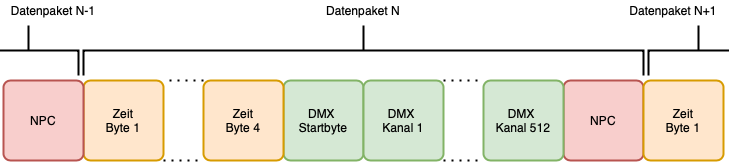
\includegraphics[width=\linewidth]{DMX-Datenformat}
		\caption{DMX-Aufnahmedaten Bytereihenfolge}
		\label{fig:DMXDatenformat}
	\end{center}
\end{figure} Geht man davon aus, dass die DMX-Datenpakete mit der maximal möglichen Frequenz von ca. 44,1\,Hz eingehen, so wird pro Minute ein Speicherplatz von:
\begin{equation}
	44,1\,Hz * 518\,Byte * 60\,s = 1370628\,Byte = 1,37\,MByte
\end{equation} auf der SD-Karte benötigt. Eine SD-Karte mit einer Kapazität von 32\,GByte bietet somit Speicherplatz für ca. 23346 Minuten aufnahme. Das entspricht einer Aufnahmedauer von etwas über 16\,Tagen. Begrenzender Faktor der maximalen Dauer einer Aufnahme stellt das $FAT$-Dateisystem dar. Es stellt nur 4-Bytes für die Angabe der Dateigröße zur Verfügung und begrenzt damit die maximale Dateigröße auf 4\,GB \cite[s. 128]{BetriebssystemeKompakt}. Eine Datei umfasst demnach maximal $2^{32}\,Byte$. Das entspricht einer maximalen kontinuierlichen Aufnahmedauer von:
\begin{equation}
	tAufnahme_{max} = \frac{2^{32}\,Byte}{518\,Byte * 44,1\,Hz * 60\,\frac{s}{min} * 60\,\frac{min}{h}} = 55,227\,h
\end{equation}
Diese Dauer sollte in den meisten Fällen ausreichend sein und könnte nur erweitert werden indem ein anderes Dateisystem verwendet wird, oder beim Erreichen der maximalen Dateigröße die Speicherung der Daten in einer zweiten Datei fortgeführt wird. 
Zusätzlich zu den DMX-Daten, werden generelle Informationen über die Aufnahme in einer separaten Datei mit der Endung $.nfo$ gespeichert. Alle Informationen werden unabhängig vom Aufnahmemodus gespeichert. Darunter befinden sich die Aufnahmedauer, die Anzahl der gespeicherten Datenpakete und das NPC-Byte.\\
\newline
\textbf{Optimierungsmöglichkeiten}\\
Die Datenpakete werden unabhängig vom Informationsgrad gespeichert, was unnötig viel Speicherplatz erfordert. Denkbar ist ein Vergleich des aktuell zu speichernden DMX-Datenpakets mit dem zuvor gespeicherten DMX-Datenpaket. Beinhaltet das zuvor gespeicherte DMX-Datenpaket die selben Informationen wie das aktuelle, so könnte die Speicherung des aktuellen Paketes übersprungen werden, da es keine neuen Informationen enthält. Dieser Vorgang benötigt allerdings Ressourcen um den Vergleich der Datenpakete vorzunehmen. Durch den Vergleich und das eventuelle wegfallen von Speicherungsvorgängen könnten widerrum Ressourcen eingespart werden.